\subsection{Конфигурации планет}

\begin{figure}[h!]
\centering
%\small
%\begin{tikzpicture}
%\fill [draw=black, fill=none,
%         postaction={decorate,decoration={raise=3pt,text along path, 
%           text={Орбита Земли}}}
%]
%  (-3, 0) arc (180:-180:3cm and 3cm);
%
%\fill [draw=black, fill=none,
%         postaction={decorate,decoration={raise=3pt,text along path,
%           text={Орбита внутренней~~~~~~~планеты}}}
%           ]
%  (-2, 0) arc (180:-180:2cm and 2cm);
%
%\fill [draw=black, fill=none,
%         postaction={decorate,decoration={raise=3pt,text along path,
%           text={Орбита внешней планеты}}}
%           ]
%  (-4, 0) arc (180:-180:4cm and 4cm);
%  
%\draw [dashed] (-2.65, -3) -- (2.65, -3);
%\draw [dashed] (0, -4) -- (0, 4);
%\draw [dashed] (0, -3) -- (-1.49, -1.33);
%\draw [dashed] (0, 0) -- (-1.49, -1.33);
%\draw [dashed] (0, -3) -- (1.49, -1.33);
%\draw [dashed] (0, 0) -- (1.49, -1.33);
%
%\filldraw [black] (0, 0) circle (1pt);
%\filldraw [black] (-1.49, -1.33) circle (1pt);
%\filldraw [black] (1.49, -1.33) circle (1pt);
%\filldraw [black] (2.65, -3) circle (1pt);
%\filldraw [black] (-2.65, -3) circle (1pt);
%\filldraw [black] (0, -3) circle (1pt);
%\filldraw [black] (0, 2) circle (1pt);
%\filldraw [black] (0, 4) circle (1pt);
%\filldraw [black] (0, -2) circle (1pt);
%\filldraw [black] (0, -4) circle (1pt);
%
%\draw (-3.7, -3.7) -- (-3.7, -3.7) node  [above,align=center,midway]{Западная\\квадратура};
%    
%\draw (3.7, -3.7) -- (3.7, -3.7) node  [above,align=center,midway]{Восточная\\квадратура};
%    
%\draw (0, -4.5) -- (0, -4.5) node  [above,align=center,midway]{Противостояние};
%
%\draw (0, 4) -- (0, 4) node  [above,align=center,midway]{Соединение};
%
%\draw (0, 0.9) -- (0, 0.9) node  [fill=white,above,align=center,midway]{Верхнее\\соединение};
%
%\draw (0, -1.75) -- (0, -1.75) node  [fill=white,above,align=center,midway]{Нижнее\\соединение};
%
%\draw (0.6, -3.4) -- (0.6, -3.4) node  [above,align=center,midway]{\ttfamily Земля};
%
%\draw (0.7, -0.2) -- (0.7, -0.2) node  [above,align=center,midway]{\ttfamily Солнце};
%
%\draw (2.3, -2.3) -- (2.3, -2.3) node  [fill=white,above,align=center,midway]{Западная\\элонгация};
%
%\draw (-2.3, -2.3) -- (-2.3, -2.3) node  [fill=white,above,align=center,midway]{Восточная\\элонгация};
%
%\end{tikzpicture}
%}
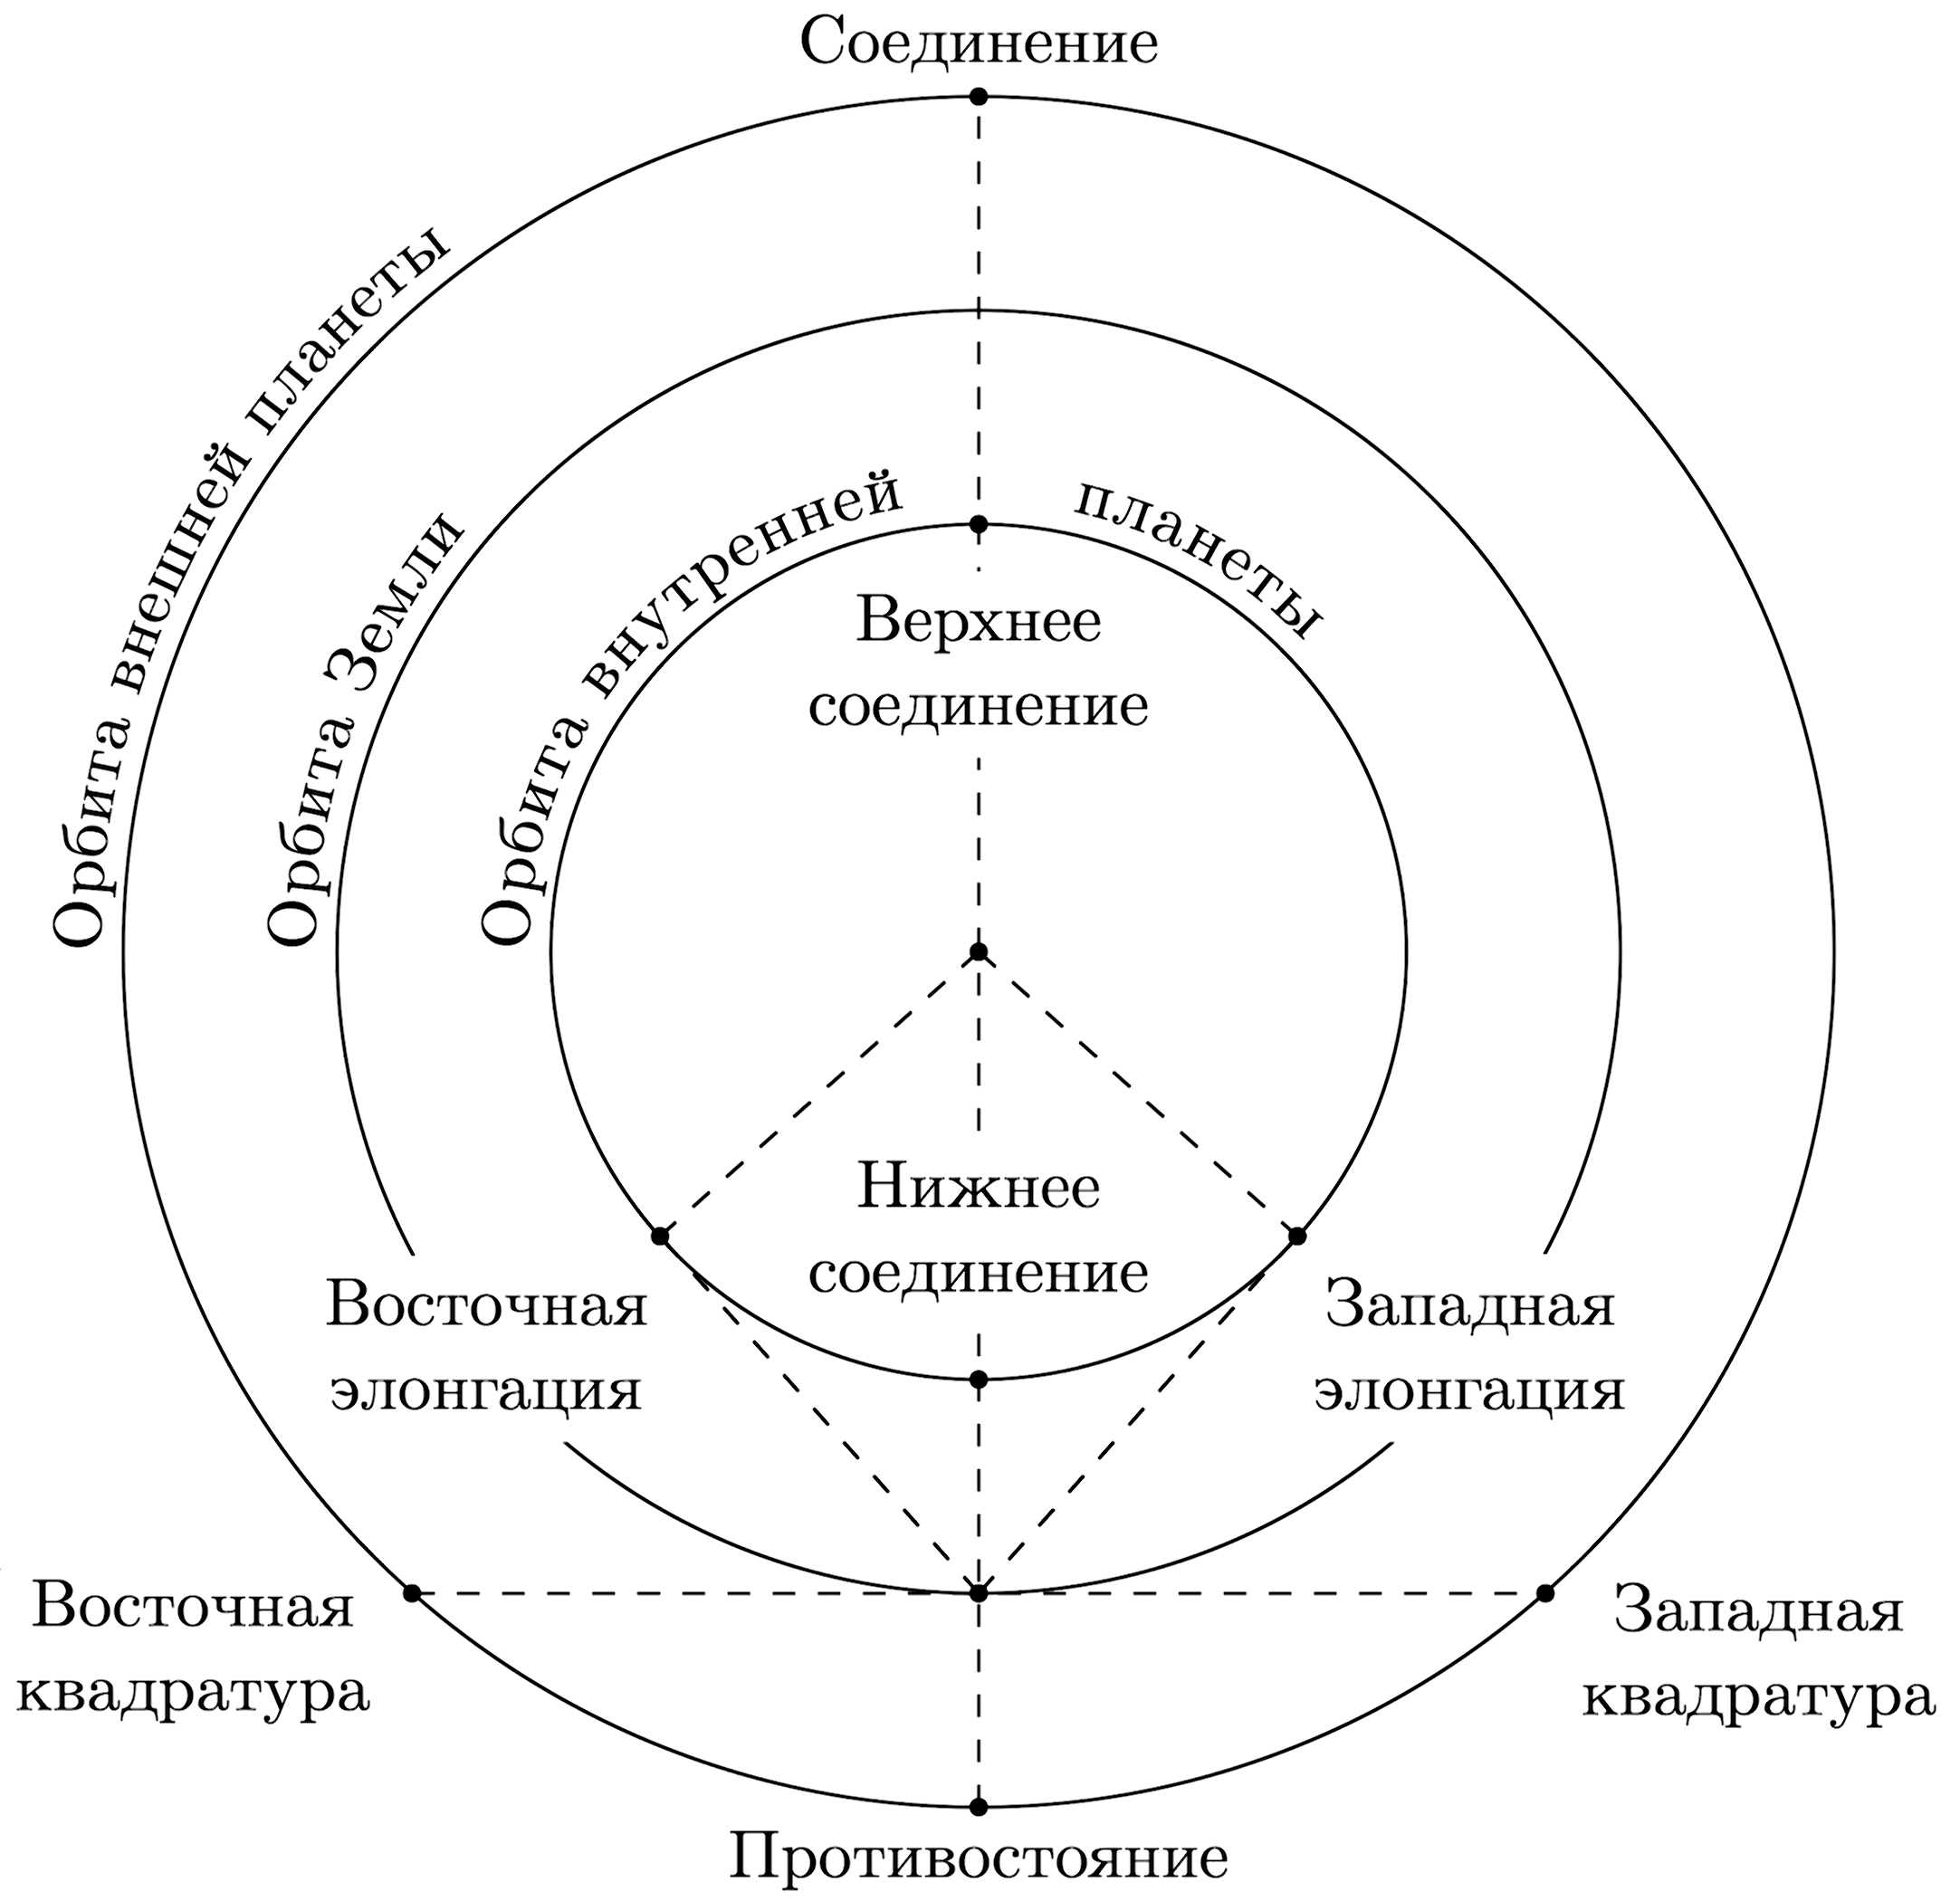
\includegraphics{planet-config}
\caption{Конфигурации планет}
\end{figure}

\term{Внутренними планетами} называются планеты, большая полуось орбиты 
$a$ которых меньше большой полуоси орбиты Земли $a_\oplus$. Отсюда следует, что 
для наблюдателя на Земле \imp{внутренними} планетами являются лишь Венера 
и Меркурий, остальные относятся к \imp{внешним}. Для таких планет выделяют 
3 основные конфигурации: \term{верхнее соединение} (1), \term{нижнее 
соединение} (2) и \term{максимальная элонгация}. Различают две максимальные 
элонгации~--- \imp{западную} (3) и \imp{восточную} (4), когда планета 
наблюдается к западу и к востоку от Солнца соответственно.

Внутренняя планета находится в \term{верхнем соединении}, когда Земля, 
Солнце и планета лежат на одной прямой, при этом планета и Земля располагаются 
по разные стороны от Солнца. Если пренебречь наклоном орбит планет к плоскости 
эклиптики, то для наблюдателя на Земле планета находится точно за Солнцем.

\term{Нижнее соединение} внутренней планеты происходит когда Земля, Солнце 
и планета, также как и в случае верхнего соединения, располагаются на одной 
прямой, но для нижнего соединения планета должна находиться между Солнцем и 
Землей. Если бы орбиты всех планет лежали в одной плоскости, тогда в момент 
каждого нижнего соединения внутренней планеты наблюдалось бы ее прохождение по 
диску Солнца для наблюдателя на внешней планете.

\term{Элонгацией} планеты называется угол Солнце -- Земля -- планета, 
отсюда очевидно, что \imp{максимальная элонгация} внутренней планеты 
наблюдается в момент, когда прямая Земля -- планета является касательной к 
орбите планеты, то есть угол Солнце -- планета -- Земля является прямым.\\

\term{Внешними планетами} называются планеты, большая полуось орбиты $a$ 
которых больше большой полуоси орбиты Земли $a_\oplus$. Для таких планет также 
существуют 3 основные конфигурации: соединение (1), противостояние (2) и 
квадратура. Квадратура бывает западная (3) и восточная (4), в какой именно 
квадратуре находится внешняя планета определяется анологично максимальной 
элонгации.

\term{Соединение} внешней планеты, подобно верхнему соединению внутренней 
планеты, наблюдается в момент, когда Солнце, Земля и планета находятся на одной 
прямой, при этом Солнце находится между планетой и Землей. В этот момент для 
наблюдателя на внешней планете Земля, являясь нижней планетой, наблюдается в 
верхнем соединении.

Аналогично, когда планета, Солнце и Земля располагаются на одной прямой, но 
Солнце и планета лежат по разные стороны от Земли, считается, что внешняя 
планета находится в \term{противостоянии}. Земля же находится в нижнем 
соединении для наблюдателя на внешней планете, наблюдаемой в противостоянии.

\term{Квадратурой} называется конфигурация, когда угол между направлениями 
на планету и Солнце (угол Солнце -- Земля -- планета) является прямым. Стоит 
заметить, что для наблюдателя на планете Земля будет наблюдаться в максимальной 
элонгации, причем если планета с Земли наблюдалась в восточной квадратуре, 
тогда Земля будет в западной максимальной элонгации и наоборот.
